\chapter{Algorithm}
\label{chapter:algorithm}

\tikzstyle{decision} = [diamond, align=center, draw=black]

\tikzstyle{block} = [rectangle, minimum width=2.5cm, minimum height=1cm, align=left, draw=black]


\section{Basis}
In our research we will extend existing work on subgraph homeomorphism. In the literature we found two existing well-defined algorithms: Xiao's algorithm `ndSHD2' \cite{XIAONODEDISJOINT} and Lingas algorithm \cite{LINGAS2009464}. Xiao's algorithm ndSHD2 is subjectively simpler: it is a depth first search in partial subgraph homeomorphism mappings (with many similarities with subgraph isomorphism algorithms) using precomputed paths. It combines attempting vertex-on-vertex mappings with attempting edge-on-path mappings. This algorithm speicifically solves the $(l,h)$ subgraph homeomorphism problem, which is the same as regular subgraph homeomorphism with the extra constraint that edges in the source graph are mapped to paths of at least $l$ edges and no more than $h$ edges. In our use case, a valid emulation mapping may have edges of any length (i.e. $l=1$ and $h=\infty$). 

In comparison, Lingas' algorithm suggests attempting their edge-path mapping strategy on every possible vertex-on-vertex mapping, without indication of which vertex-on-vertex mappings are likely to result in finding subgrapp homeomorphim.

Because Xiao's algorithm's simplicity and coverage of each aspect of the algorithm's process, it is suitable for FPGA use cases and optimisations. However, because of the algorithm's exponential space requirements, we will devise a similar (less space-demanding) algorithm using Xiao's algorithm as inspiration. In this algorithm we will compute paths at runtime instead of as precomputation, and as such call it RTSH (Run Time Subgraph Homeomorphism).

To understand our algorithm better, let us first examine what the output is supposed to be. The algorithm should, given two graphs, not just indicate whether the latter graph has a subgraph homeomorphism of the former, but also indicate what subgraph homeomorphism that is. More formally, we need to solve the \textit{certification} problem rather than the \textit{decision} problem. This certification indicates to which target graph vertex each source graph vertex is mapped and to which target graph path each source graph edge is mapped such that the entire mapped source graph is a subgraph of the target graph. This is what we will from now on refer to as the \textbf{mapping}. If, during the execution, the mapping is not yet complete, i.e. it does not have a target for some source graph vertex or edge, we refer to it as the \textbf{partial mapping}.

%ndshd2 old
\begin{algorithm}
\DontPrintSemicolon
\SetAlgoLined
\LinesNumbered
\textbf{Inputs: } the current vertex-vertex partial mapping $\mathit{vmap}$, the current edge-path $\mathit{emap}$ partial mapping\\
\textbf{Outputs: } \textit{found}, indicating whether a valid subgraph homeomorphism has been found.\\

\If {$s$ is complete} {
	\Return true\;
}

$\mathit{found} \longleftarrow \mathit{false}$

 \While{$!\mathit{found} \land \exists$ valid node/edge-path mapping pair}{

\If{$\mathit{hasUnmatchedEdge}()$} {
	$(e_S, p_T) \longleftarrow \mathit{GetNextEdgePathPair}()$\;
  	$\mathit{emap} \longleftarrow \mathit{emap} \cup \{(e_S, p_T)\}$\;
  	$\mathit{found} \longleftarrow \mathit{RTSH}(\mathit{vmap}, \mathit{emap})$\;
  \If{found} {
  	\Return true\;
  }
  $\mathit{emap} \longleftarrow \mathit{emap} \cap \{(e_S, p_T)\}$\;
} \Else {
	$(v_S, v_T) \longleftarrow \mathit{GetNextNodePair}()$\;
  	$\mathit{vmap} \longleftarrow \mathit{vmap} \cup \{(v_S, v_T)\}$\;
  	$\mathit{found} \longleftarrow \mathit{RTSH}(\mathit{vmap}, \mathit{emap})$\;
  \If{found} {
  	\Return true\;
  }
  	$\mathit{vmap} \longleftarrow \mathit{vmap} \cap \{(v_S, v_T)\}$\;
}

 }
 \Return false\;
 \caption{Basis of RTSH}
 \label{algorithm:ndSHD2Old}
\end{algorithm}






Our base algorithm is shown in Algorithm \ref{algorithm:ndSHD2Old}. It is a form of depth first search in a partial mapping search space that attempts- and backtracks vertex-on-vertex mappings and edge-on-path mappings.

In our literature study, we found that the core of many subgraph isomorphism algorithms\footnote{Ullman, VF, VF2, VF2+, VF2++, UI, Fast-ON, L2G, Cheng, QuickSI, GraphQL, ILF, TurboISO, Glassgow, CLF-Match, RI, RI-DS, McGregor, LAD, PathLAD} is a form of similar DFS state space exploration where the states consist of partial vertex-to-vertex mappings. In subgraph isomorphisms, the edge-to-edge mapping is elementary by performing the vertex mapping on the edge source and target to obtain the target edge. With the subgraph homeomorphism algorithm such as ours and Xiao's, an additional mapping from $E_S$ to the path set of $G_T$ is needed.

The algorithm starts with an empty partial mapping, and starts mapping source graph vertices to target graph vertices. Whenever both vertices of a source graph edge have been matched, the algorithm finds some path (according to some path iteration method) between the mapped edge source and target in the target graph that is internally disjoint from target graph vertices already used in the partial mapping. The algorithm prioritizes extending the matching with an edge-path pair over extending it with a vertex-vertex pair. Whenever no such path or vertex exists, the algorithm undoes (backtracks) the last matching step taken and tries a different alternative. %Whenever a partial match is extended with a vertex-vertex pair or with an edge-path pair the search space is refined using a pruning strategy implemented by the $wouldPrune$ call. This method filters out future path candidates from a path storage and from a vertex storage according to zero-domain N-reachability pruning (see Chapter \ref{chapter:pruning} for definitions). This removes path candidates and vertex candidates that can provably not be part of any valid subgraph homeomorphism mapping.

The algorithm in Xiao's paper is comparable to our base algorithm we present here, and leaves out some specific ordering details that may be relevant for the algorithm's performance. We specify our own orderings in Sections \ref{sec:sourceOrder}, \ref{sec:targetOrder}. We will explain what ordering of paths we use in Section \ref{sec:pathIterationShort}. We will introduce some optimisations to the algorithm in Section \ref{sec:optimisations}.

\section{How to choose vertex-vertex pairs}
There are different ways to choose which vertex-vertex pair to try adding to the partial mapping first, and which only to try adding after other attempts have failed. These methods can be divided into three categories:

\begin{enumerate}
\item Choose a source graph vertex first using some heuristic, then attempt all target graph vertex candidates using another heuristic.
\item Choose a target graph vertex first using some heuristic, then attempt all source graph vertex candidates using another heuristic.
\item Choose a source vertex-target vertex with high heuristic first, then attempt all other pairs.
\end{enumerate}

While the strategy used does not affect the vertex-on-vertex mapping state space, it can affect the average-case performance. Strategy 3, for example, uses combined heurstics that may be more powerful. The disadvantage of it requires $O(|V_s|*|V_t|)$ heuristic computations before the first pair is obtained. If these computations are done beforehand the heuristic cannot take the current partial mapping into account and is likely to be weak. Is this computation is done at each step in the search process, it introduces considerable delay.

Strategies 1 and 2, on the other hand, require only $O(|V_s|+|V_t|)$ heuristic calculations to be made before obtaining a candidate pair. We choose strategy 1 with a source graph vertex heuristic that is precomputed and provide two heuristics for target graph vertices, one of which is precomputed and one of which is calculated run-time.

\section{Source graph vertex order}
\label{sec:sourceOrder}
The source graph vertex order is the order in which source graph vertices are added to the partial mapping. For example, if $s_1 \prec_M s_2$ in this ordering, then a pair with $s_2$ and some target graph vertex will only be added to the partial mapping if a pair with $s_1$ is already in it within the context of a partial matching $M$. If this ordering depends on $M$, it has to be calculated at run-time. If it does not, it only has to be precomputed once.

Xiao does not specify a source graph vertex order. Instead, we will use a high-performance ordering technique from the subgraph \textit{isomorphism} domain. From performance comparisons (see Appendix \ref{app:algorithmHistory}) we extract that the best performing algorithm that adheres to partial mapping search for subgraph isomorphism is RI-DS \cite{RIalgorithm}. In our literature study, we found no evidence a faster algorithm exists. This ordering does not depend on $M$, and thus we will precompute the entire ordering.

To describe the ordering process of RI-DS, let us provide a few definitions:

\begin{defn}[predecessors and successors]
Given two graphs $G=(V, E, L)$ and some vertex $v \in V$, their predecessors and successors are defined as follows:

$\mathit{succ}(v) := {v' \in V . (v, v') \in E}$

$\mathit{pred}(v) := {v' \in V . (v', v) \in E}$
 
\end{defn}

\begin{defn}[neighbour set]
If some $v\in V$, then $\mathit{neighbours}(v):= \mathit{succ}(v) \cup \mathit{pred}(v)$.
\end{defn}

%\begin{defn}[E for sets of vertices]
%If some $S\subseteq V$, then $E(S):=\bigcup\limits_{v \in S} E(v)$.
%\end{defn}


The algorithm RI-DS obtains a static source graph vertex ordering using a greedy algorithm called ``GreatestConstrainedFirst". This algorithm starts with an empty list and adds vertices to the end of the list, resulting in an ordering in which vertices earlier in the list are prioritized. It starts with a list $\mu$ containing only the source graph vertex with the highest degree, i.e. $s\in V_S$ where $|\mathit{neighbours}(s)|$ is highest. Then, each source graph vertex not yet in the list is assigned three scores $N_1$, $N_2$ and $N_3$. $N_1(s)$ is the number of neighbours of $s$ that are already in the list (i.e. $|\{s' | s' \in \mathit{neighbours}(s) \land s' \in \mu\}$|). $N_2(s)$ is the number of neighbours of $s$ that are not in the list themselves, but do have a neighbour in the list (i.e. $|\{s' | s' \in \mathit{neighbours}(s) \land s' \not \in \mu \land \mathit{neighbours}(s') \cap \mu \neq \emptyset\}$|). $N_3(s_x)$ is the number of all remaining neighbours of $s$ (i.e. $|\{s' | s' \in \mathit{neighbours}(s) \land s' \not \in \mu \land \mathit{neighbours}(s_y) \cap \mu = \emptyset\}$|). It selects each vertex $s$ of which $N_1(s)$ is greatest. Ties are broken with the greatest $N_2$-value, and any remaining ties are broken with the greatest $N_3$-value. Any remaining ties are broken randomly. The selected vertex is added to the back of the list, and the process repeats. This continues until every vertex has been added to the list.

The result of this ordering is that consequent vertices have many edges with vertices earlier in the ordering. Xiao established that matching edges as soon as possible (rather than matching vertices first) results in a faster algorithm. Using an order that allows early placement of edges such as GreatestConstrainedFirst should accoring to Xiao result in fast execution.
\section{Target graph vertex order}
\label{sec:targetOrder}

The target graph vertex order is the order in which target graph vertices are added to the partial mapping. For example, if $t_1 \prec t_2$ in this ordering, then a pair with $t_2$ and some source graph vertex $s_x$ will only be added to the partial mapping if the pair $(s_x, t_1)$ was already proved infeasible. Xiao does not describe a specific target graph vertex order.

We found one subgraph isomorphism algorithm that describes a specific target graph vertex order, being Glasgow \cite{McCreesh2015}. In this algorithm, target graph vertices with higher degree are prioritized. Since this does not depend on the chosen source graph vertex or on the current partial matching, this order can be precomputed, introducing only linear complexity. Formally, when some source graph vertex $s$ needs to be matched, target graph vertices are chosen using the following metric, choosing vertices with lower metric values first:

$$\mathit{metric}_\mathit{degree}(s, t)=-|\mathit{neighbours}(t)|$$

Another option (that is not attempted by subgraph homeomorphism algorithms before) is to take the current partial mapping into account. Using a degree-based or random target graph vertex order will result in chosen target graph vertices to be independent of already used target graph vertices, potentially requiring many resouces to reach. However, we can use information from the current partial mapping to obtain better candidates: since we know the chosen source graph vertex and thus which edges will be mapped after this vertex-vertex pair, we can choose our target vertex such that the paths associated with these edges are as short as possible.

Whenever we need to match some source graph vertex $s$, This distance-based method will choose target vertices first that have the lowest distance to the source graph vertex' neighbours that are already in the partial matching. The result is that fewer number of vertices need to be used as intermediate vertex in the paths associated with the edges to those neighbours. The disadvantage of this method is that it requires runtime usage of a computionally expensive shortest path algorithm to choose a target graph vertex candidate. The shortest path algorithm can be cached, which reduces the number of computations needed after backtracking but introduces quadratic ($O(|V_s|*|V_t|)$) space usage (we implement this with- and without caching). Formally, when some source graph vertex $s$ needs to be matched, $t_x$ are chosen using the following metric, choosing vertices with lower metric values first:


$$\mathit{metric}_\mathit{distance}(s, t)=\sum_{s' \in E(s)} \begin{cases}
|\mathit{shortestPathUndirected}(M(s'), t)| & s' \prec_\mu s\\
0 & s \prec_\mu s'
\end{cases}$$

Here, $M$ is the current partial mapping and $\mu$ is the source graph vertex order. We implemented both methods to use in our algorithm.

\section{Path iteration}
\label{sec:pathIterationShort}
In subgraph isomorphism, edge-on-edge mappings can be trivially computed from vertex-on-vertex mappings. However, in subgraph homeomorphism a source graph edge may be mapped on many target graph path candidates (all starting- and ending at the same two vertices). Therefore, we cannot extract the order in which to try out paths from subgraph isomorphism. Instead, we implemented different methods to iterate over paths to try:

\begin{itemize}
\item \textbf{K-path -} Try all loopless paths from shortest to longest, avoiding unusable vertices in the existing partial mapping. We use Yen's algorithm \cite{YensAlgorithm} for this. Faster and more recent algorithms exist \cite{Hershberger, Brander1996} but lack public implementations.

\item \textbf{DFS -} Search for paths using depth first search from the start vertex, choosing arbitrary directions at each vertex and avoiding unusable vertices in the existing partial mapping.

\item \textbf{Greedy DFS (graph distance) -} Search for paths using greedy depth first search, choosing the direction closest to the goal vertex first (avoiding unusable vertices in the existing partial mapping). We implement both a variant that precomputes all shortest paths and a variant that calculates at run-time which direction to choose (without caching).

\item \textbf{Greedy DFS (informed graph distance) -} Search for paths using greedy depth first search, choosing the direction closest to the goal vertex along a path that avoids unusuble vertices first (avoiding unusable vertices in the existing partial mapping). We compute run-time which direction to choose.

\item \textbf{Control point -} Select increasingly many `control points' (from $0$ to $|V|$) randomly in the target graph that must be in the path in a specific order, then connecting them by a shortest path algorithm that avoids unusable vertices in the existing partial mapping. We implemented this with a recursive algorithm in which a replacement of some control point is only attempted if all control points \textit{earlier} in the control point order have been attempted.\footnote{To avoid duplicate paths, any path that can be generated with fewer control points is skipped. Furthermore, any control point configuration where shifting some control point towards the goal vertex along the path results in the same path is skipped.}
\end{itemize}

These methods provide for each two vertices in a graph each path connecting them exactly once. The space requirements for each method are shown in Table \ref{tab:iterator-spacerequirements}, and examples of paths returned by them are shown in Appendix 2.

\begin{table}
\centering
\begin{tabular}{|l|l|}
\hline
\textbf{Path iterator} & \textbf{Space complexity} \\ \hline
K-Path                 & $O(|V|!)$                 \\ \hline
DFS                    & $O(|V|)$                  \\ \hline
Greedy DFS             & $O(|V|^2)$                \\ \hline
Control point          & $O(|V|)$                  \\ \hline
\end{tabular}
\caption{Worst-case \textbf{space} complexity of each path iteration strategy. The \textbf{computational} requirements of each method change in different ways for subsequent calls.}
\label{tab:iterator-spacerequirements}
\end{table}


\section{Optimisations}
\label{sec:optimisations}
Since our use case entails finding subgraph homeomorphisms in relatively large graphs, any optimisation possible improves our chances of finding FPGA emulation mappings within reasonable time. Therefore, in addition to implementing ordering parameters for the ndSHD2 algorithm, we implement some optimisations and individually evaluate them. The algorithm with optimisations implemented is shown in Algorithm \ref{algorithm:ndSHD2-prune}.

\subsection{Refusing long paths}
\label{sec:refusinglongerpaths}
Since path iterators may provide any valid path to map an edge to during the matching process, they may also provide paths that take up unnecessarily many resources. Specifically, they take up so many resources that with a subset of the vertices and edges of that path, a shorter path can be formed. Formally, some path $t_0\dots t_n$ is ``unnecessarily long" iff:


%$\exists p' \in P_T . first(p') = first(p) \land last(p') = last(p) \land intermediate(p') \subset intermediate(p)$
$\exists t_i \in t_0\dots t_{n-2} . \exists t_j \in t_{i+2}\dots t_n . (t_i, t_j) \in E_T$

With this optimisation, such paths are skipped by path iterators. Examples of this effect are shown in Appendix \ref{app:pathIteratorExamples}, Figures \ref{fig:pathexamples-dfs}
 and \ref{fig:pathexamples-greedydfs}.

\subsection{Runtime Pruning}
Some subgraph isomorphism algorithms \cite{Cordella2004, McCreesh2015} prune the search space during the search using some detection method of dead search paths. Xiao's algorithm does this as well. For our algorithm, we will implement different types of pruning methods of varying strength (dead search branch detection capability) and computational requirements..

\subsection{Contraction}
\label{sec:contraction}
The source graph of a homeomorphism case will often contain vertices that have exactly one incoming edge and one outgoing edge. In FPGAs, for example, these could be transistors or ports of components. These vertices do topologically nothing but serve as an edge; therefore they may also be thought of as an edge, where the edge source is the vertex' predecessor and the edge target is the vertex' successor. When we use the word contraction, we mean surpressing all such vertices in the virtual FPGA and replacing them with a single edge, as illustrated in Figure \ref{fig:contraction-basic}. This process transforms the source graph $S$ into the smallest graph $S_{cont}$ that is topologically equivalent to $S$. This may be a multigraph or a graph that contains self-loops. If a subgraph homeomorphism exists from $S$ to some target graph $T$, then there also exists a subgraph homeomorphism from $S_{cont}$ to $T$ (a proof is given in Appendix \ref{proof:contractionHomeo}). The optimisation `contraction' searches for a homeomorphism between $S_{cont}$ and the $T$ instead of finding one between $S$ and $T$. Because this involves a smaller source graph, it also involves a smaller search space. Note that we do not change/contract the target graph representing the concrete FPGA.

The process of finding a homeomorphism from $S_{cont}$ to $T$ is slightly different from what normal. This is because while every homeomorphism from $S$ to $T$ can be deduced to a homeomorphism between $S_{cont}$ and $T$ (by contraction of vertices and concatenation of paths), not every homeomorphism from $S_{cont}$ and $T$ allow a homeomorphism from $S$ to $T$ to be inferred. An example is the case where $S_{cont}$ is isomorphic to $T$ and $S$ subdivides a single edge of $S_{cont}$: there exists a subgraph homeomorphism from $S_{cont}$ to $T$ since they are isomorphic, but there is no subgraph homeomorphism from $S$ to $T$. Because of this, we need to adapt the subgraph homeomorphism search process such that it only finds subgraph homeomorphisms from which we \textit{can} infer a subgraph homeomorphism from $S$ to $T$.

When we apply contraction to replace a series of edges $E$ separated by contractable vertices by a single edge $e$ with the intermediate vertices contracted, we save the label sets for each intermediate vertex in $E$ in the order that they appear (following the direction of $e$) before starting the search algorithm. 

During edge-path matching in the partial mapping search, we may need to map an edge $(u, v)$ that contains contracted vertices. For each edge $\in E_{cont}$ with the same source- and target vertex we recall their lists of contracted label sets. Each time we find a path candidate for $(u, v)$ we check compatibility of that path with each of those lists of label sets. We then retrieve all other paths already found for edges with this source- and target and use an all-different constraint (see Section \ref{sec:alldifferent}) to verify that each edge $\in E_{cont}$ has a compatible path. Whenever the number of paths is smaller than the number of edges (i.e. paths still need to be found futher in the partial mapping search), we assume paths that are compatible with every list of label sets.

If the all-different constraint fails, it implies that from the current partial mapping we cannot find paths that emulate the contracted vertices, and we backtrack. If the all-different constraint succeeds, finding a subgraph homeomorphism is still possible and we continue.

This optimisation introduces some delay since the algorithm needs to check compatibility between label set sequences and paths and solve an all-different constraint. However, it also saves time since it reduces the source graph's size. 

\subsubsection{Contraction for undirected graphs}
Although we are focued on directed graphs in our algorithm, it is interesting to note that each optimisation is also applicable to undirected graphs, including contraction. Contraction can be applied to undirected graphs by temporarily applying a uniform direction to each chain of 2-degree vertices in the source graph and then applying directed contraction, after which the edges may lose their direction again. Then, during the compatibility checking process we perform the same procedure, making sure the list of label sets is checked in the correct direction, i.e. for each temporarily directed edge $(u, v) \in E_{cont}$ and partial mapping $M$, the path $M(u, v)$ in $T$ should be checked in the direction from $M(u)$ to $M(v)$.

\begin{figure}
\begin{subfigure}{.5\textwidth}
  \centering
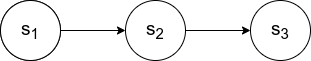
\includegraphics[width=0.8\linewidth]{images/contraction/whatisit1.png}
  \caption{Part of a source graph that may be contracted}
\end{subfigure}
\begin{subfigure}{.5\textwidth}
  \centering
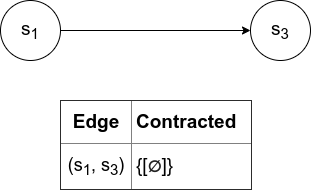
\includegraphics[width=0.8\linewidth]{images/contraction/whatisit2.png}
  \caption{The result of contraction}
\end{subfigure}
\caption{Contraction applied to vertex $s_2$, a vertex with indegree 1 and outdegree 1. During contraction, we save that a single vertex has been contracted with an empty label set.}
\label{fig:contraction-basic}
\end{figure}


\begin{figure}
\begin{subfigure}{.55\textwidth}
  \centering
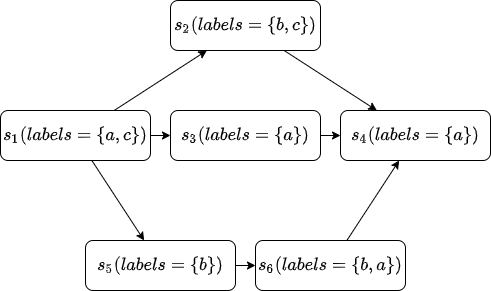
\includegraphics[scale=0.5]{images/contraction/after2.png}
  \caption{A source graph before contraction}
\end{subfigure}
\begin{subfigure}{.45\textwidth}
  \centering
  % include second image
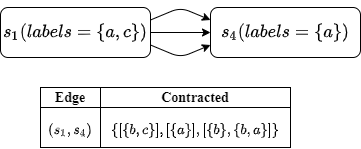
\includegraphics[scale=0.6]{images/contraction/before2.png}
  \caption{The same source graph after contraction.}
\end{subfigure}
\caption{Contraction applied to a source graph with labels. With this optimisation, 3 fewer vertices and 4 fewer edges need to be mapped. During contraction, we save the label sets of the contracted vertices in the order of the contracted path.}
\label{fig:contraction}
\end{figure}





\section{Avoiding unintended current flow}
\label{sec:unintendedcurrent}
As mentioned in Chapter \ref{chapter:models}, the concrete FPGA may contain transistors that are always enabled, i.e. cannot be configured to block the flow of electrical current and function as a diode. If we would ignore this property of transistors, we may obtain a mathematically sound subgraph homeomorphism that does not include every unconfigurable transistor from the target graph in its mappings. If some unconfigurable transistor (or a sequence of them) connect two vertices in the target graph that \textbf{are} part of the mapping, then the subgraph homeomorphism does not describe a valid emulation: if the state of two components are independent in the virtual FPGA they should be independent in the concrete FPGA as well to preserve the semantics of the FPGA configuration. An example of this effect is given in Figure \ref{fig:unconfigurableExample}. To avoid this issue, we propose two measures:


\begin{figure}

  \centering
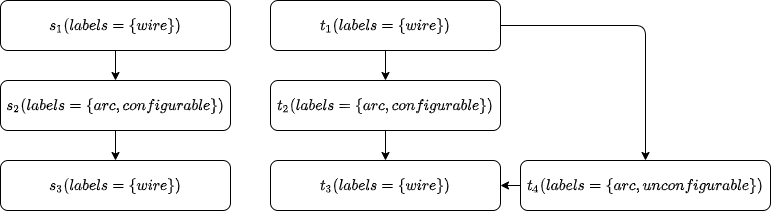
\includegraphics[scale=0.6]{images/contraction/unconfigurableExample.png}

\caption{An example of a pair of FPGAs with an unconfigurable transistor in the concrete FPGA. There exists a mathematically sound subgraph homeomorphism $(\{s_1 \to t_1, s_2 \to t_2, s_3 \to t_3\}, \{(s_1, s_2) \to [(t_1, t_2)], (s_2, s_3) \to [(t_2, t_3)]\})$. However, a configuration in which the virtual FPGA transistor $s_2$ is disabled cannot be translated to a configuration in the target FPGA with the same semantics. While $t_2$ can be configured to be disabled, the electrical current can always flow from $t_1$ to $t_3$ through $t_4$. The algorithm should avoid finding subgraph homeomorphisms like these.}

\label{fig:unconfigurableExample}
\end{figure}

\subsection{Avoiding unintended current flow from/to paths}
\label{sec:unintendedcurrent-path}
Our first remedy is to avoid adding target graph vertices to the partial mapping that are connected to some path already present in the edge-path partial mapping through unconfigurable vertices. 

These vertices can get electrical currents whenever it flows though the path, possibly breaking the program's semantics. Therefore, we avoid adding these vertices to the partial mapping by deleting them from the graph in search branches that include the corresponding paths. Deleting them prevents us from adding them to the partial mapping and having our semantics changed. 

More formally:

Let $\mathit{unconfigurable}\in (V_T \times V_T)$ be the relation between two vertices if they are connected through a vertex representing a unconfigurable transistor, i.e:

\vspace{10pt}

\begin{center}
\begin{tabular}{ll}
$\mathit{unconfigurable} := \{(t_1, t_2) \in (V_T \times V_T) | \exists u \in (V_T \setminus \{t_1, t_2\}) .$&$\mathtt{UNCONFIGURABLE} \in L(u) \land$\\
&$\mathtt{CONFIGURABLE} \not \in L(u) \land$\\
&$\{(t_1, u), (u, t_2)\} \subseteq E_T\}$
\end{tabular}
\end{center}

\vspace{10pt}
Let $\mathit{unconfigurable}^*$ be the symmetric closure of the transitive closure of $\mathit{unconfigurable}$. Then, whenenever we add an edge-path pair $(e, p)$ to the partial mapping, we delete each vertex $x$ for which $\exists v \in \mathit{intermediate}(p) . (x, v) \in \mathit{unconfigurable}^*$.  Whenever $(e, p)$ is later removed from the partial mapping, each such vertex and their edges is added back to the target graph. After all, these vertices \textit{are} allowed to be in our mapping if $p$ is not.


\subsection{Avoiding unintended current flow between mapped vertices}
\label{sec:unintendedcurrent-vertex}
Our second remedy is to avoid adding target graph vertices to the partial mapping that are connected to some target graph vertex already present in the vertex-vertex partial mapping through unconfigurable vertices. Allowing this could result in wires in the concrete FPGA receiving an electrical current that is not part of the program's semantics.

We also do this by deleting vertices: this time, whenever we add a vertex-vertex pair $(s, t)$ to the partial mapping, we delete each vertex $x$ for which $(x, t) \in \mathit{unconfigurable}^*$. Whenever $(s, t)$ is later removed from the partial mapping, each such vertex and their edges is added back to the target graph.

\newfloat{myalgo}{tbhp}{mya}
\newenvironment{Algorithm}[2][tbh]%
{\begin{myalgo}[#1]
\centering
\begin{minipage}{#2}
\begin{algorithm}[H]}%
{\end{algorithm}
\end{minipage}
\end{myalgo}}


%ndshd2-contract
\begin{Algorithm}{18cm}
\DontPrintSemicolon
\SetAlgoLined
\LinesNumbered
\textbf{Inputs: } the source graph $G_S$ and the target graph $G_T$\\
\textbf{Outputs: } Whether a valid subgraph homeomorphism has been found.\\
\If{contraction} {
	$G_S, \mathit{chains} \longleftarrow \mathit{contract}(G_S)$ \tcp*[hr]{sec. \ref{sec:contraction}}
}
 \Return $\mathit{RTSH*}(\mathit{vmap}$, $\mathit{emap}$)\tcp*[hr]{Algorithm \ref{algorithm:ndSHD2-ext}}\;
 \caption{RTSH}
 \label{algorithm:ndSHD2-prune}
\end{Algorithm}

\mathchardef\mhyphen="2D % Define a "math hyphen"

%ndshd2 new
\begin{Algorithm}[t]{18cm}
\DontPrintSemicolon
\SetAlgoLined
\LinesNumbered
\textbf{Inputs: } the current vertex-vertex partial mapping $\mathit{vmap}$, the current edge-path $\mathit{emap}$ partial mapping\\
\textbf{Outputs: } \textit{found}, indicating whether a valid subgraph homeomorphism has been found. \color{red}if has unmatched edge: \ref{line:ifHasUnmatchedEdge} unnecessarily long \ref{line:unneccesarilyLong} contraction check \ref{line:contractionCheck} get next edge path pair \ref{line:getNextEdgePathPair} get next vertex pair \ref{line:getNextVertexPair} prune path \ref{line:prunePath} prune vertex \ref{line:pruneVertex} recursive call path \ref{line:recursivePath} recursive call vertex \ref{line:recursiveVertex} add to emap \ref{line:addToEmap} add to vmap \ref{line:addToVmap} return true recursive path \ref{line:returnRecursivePath} return true recursive vertex \ref{line:returnRecursiveVertex} remove from cover path \ref{line:removeFromCoverPath} return true first time \ref{line:returnTrueFirstTime}\color{black}\\

\If {$s$ is complete} {
	\Return true\label{line:returnTrueFirstTime}\;
}

$\mathit{found} \longleftarrow \mathit{false}$

 \While{$!\mathit{found} \land \exists$ valid node/edge-path mapping pair}{

\If{\label{line:ifHasUnmatchedEdge}$\mathit{hasUnmatchedEdge}()$} {
	$(e_S, p_T) \longleftarrow \mathit{GetNextEdgePathPair}()$\label{line:getNextEdgePathPair}\;
	\If(\tcp*[f]{sec. \ref{sec:contraction}}){$\mathit{isUnnecessarilyLong}(p_T) \lor$ \label{line:unneccesarilyLong} \tcp*[r]{sec. \ref{sec:refusinglongerpaths}} $\mathit{wouldPrune}(\mathit{vmap}, \mathit{emap} \cup \{(e_S, p_T)\}) \lor$\label{line:prunePath}\tcp*[r]{algo. \ref{algorithm:wouldPrune-ext}}$(\mathit{contraction} \land \lnot \mathit{chainsCompatible}(\mathit{emap}, \mathit{from}(e_S), \mathit{to}(e_S), p_T))$\label{line:contractionCheck}} {
  		\textbf{continue}\;
  	}
	$V_T \longleftarrow V_T \setminus \mathit{unconfigurableCover}(\mathit{intermediate}(p_T))$\label{line:removeFromCoverPath}\hspace{3.72cm}\tcp*[f]{sec. \ref{sec:unintendedcurrent-path}}\;  	
  	
  	$\mathit{emap} \longleftarrow \mathit{emap} \cup \{(e_S, p_T)\}$\label{line:addToEmap}\;
  	$\mathit{found} \longleftarrow \mathit{RTSH*}(\mathit{vmap}, \mathit{emap})$\label{line:recursivePath}\;
  \If{found} {
  	\Return true\label{line:returnRecursivePath}\;
  }
  $\mathit{emap} \longleftarrow \mathit{emap} \cap \{(e_S, p_T)\}$\;
  $V_T \longleftarrow V_T \cup \mathit{unconfigurableCover}(\mathit{intermediate}(p_T))$\hspace{3.65cm}\tcp*[f]{sec. \ref{sec:unintendedcurrent-path}}\;	
} \Else {
	$(v_S, v_T) \longleftarrow \mathit{GetNextNodePair}()$\label{line:getNextVertexPair}\;
	\If(\tcp*[f]{algo. \ref{algorithm:wouldPrune-ext}}){\label{line:pruneVertex}$\mathit{wouldPrune}(\mathit{vmap} \cup \{(v_S, v_T)\}, \mathit{emap})$} {
  		\textbf{continue}\;
  	}
  	$V_T \longleftarrow V_T \setminus \mathit{unconfigurableCover}(v_T)$\hspace{6.3cm}\tcp*[f]{sec. \ref{sec:unintendedcurrent-vertex}}\;  
  	$\mathit{vmap} \longleftarrow \mathit{vmap} \cup \{(v_S, v_T)\}$\label{line:addToVmap}\;
  	$\mathit{found} \longleftarrow \mathit{RTSH*}(\mathit{vmap}, \mathit{emap})$\label{line:recursiveVertex}\;
  \If{found} {
  	\Return true\label{line:returnRecursiveVertex}\;
  }
  	$\mathit{vmap} \longleftarrow \mathit{vmap} \cap \{(v_S, v_T)\}$\;
  	$V_T \longleftarrow V_T \cup \mathit{unconfigurableCover}(v_T)$\hspace{6.3cm}\tcp*[f]{sec. \ref{sec:unintendedcurrent-vertex}}\;	
}

 }
 \Return false\;
 \caption{RTSH*}
 \label{algorithm:ndSHD2-ext}
\end{Algorithm}


%wouldPrune new
\begin{algorithm}
\DontPrintSemicolon
\SetAlgoLined
\LinesNumbered
\textbf{Inputs: } the current vertex-vertex partial mapping $\mathit{vmap}$, the current edge-path $\mathit{emap}$ partial mapping\\
\textbf{Outputs: } whether pruning should be applied.\\

\If {$\mathit{serialPruning} \lor (\mathit{parallelPruning} \land \mathit{pruningThreadFailed})$} {
	$\mathit{domains} \longleftarrow \mathit{filterDomains}(\mathit{vmap}, \mathit{emap})$\;
} \ElseIf {$\mathit{cachedPruning}$} {
	$\mathit{domains} \longleftarrow \mathit{updateDomains}(\mathit{vmap}, \mathit{emap})$\;
} \Else {
	\Return false\;
}
$\mathit{toPrune} \longleftarrow \text{false}$\;
\If {ZeroDomain} {
	$\mathit{toPrune} \longleftarrow \emptyset \in \mathit{values}(\mathit{domains})$\hspace{6cm}\tcp*[f]{sec. \ref{sec:zerodomainpruning}}\;
} \ElseIf {AllDifferent} {
	$\mathit{toPrune} \longleftarrow \lnot \mathit{satisfiesAllDifferent}(\mathit{domains})$\hspace{4.2cm}\tcp*[f]{sec. \ref{sec:alldifferent}}\;
}

\If {$\mathit{parallelPruning} \land \lnot \mathit{toPrune}$} {
	$\mathit{pruningThreadFailed} \longleftarrow \text{false}$\;
	\tcc{Set to \textbf{true} by pruning thread whenever it would prune the partial mapping that it queried from the main thread.}
}

\color{black}
\Return $\mathit{toPrune}$\;
 \caption{wouldPrune}
 \label{algorithm:wouldPrune-ext}
\end{algorithm}


%chainsCompatible
\begin{algorithm}
\SetKwFor{RepTimes}{repeat}{times}{end}
\SetAlgoLined
\LinesNumbered
\textbf{Inputs: } the current edge-path $\mathit{emap}$ partial mapping, the source vertex $v_s$ and the target vertex $v_t$ of the edge to be added, the path to be associated with that edge $p$\\
\textbf{Outputs: } Whether we need are safe to continue (true) or need to backtrack (false) due to contraction compatibility issues.\\
$\mathit{labelsetSequences} \longleftarrow \mathit{chains}(v_s, v_t)$\;
$\mathit{pathBag} \longleftarrow \{\mathit{emap}(e) . e \in E_S \land \mathit{from}(e)=v_s \land \mathit{to}=v_t \} \cup \{p\}$\;

$\mathit{edgesToGo} \longleftarrow |\{e \in E_S . e \not \in \mathit{emap} \land \mathit{from}(e)=v_s \land \mathit{to}(e)=v_t\}|$

\RepTimes {$\mathit{edgesToGo}$} {
		$\mathit{pathBag}\longleftarrow \mathit{pathBag} \cup \{\top\}$\;	
}

\For {$\mathit{seq} \in \mathit{labelsetSequences}$} {
	$\mathit{domain}(\mathit{seq})\longleftarrow \{p' \in \mathit{pathBag} . \mathit{containsSubSequence}(\mathit{seq}, p')\}$\;
}

\Return $\mathit{satisfiesAllDifferent}(\mathit{domains})$\;

 \caption{chainsCompatible}
 \label{algorithm:chainsCompatible}
\end{algorithm}


%containsSubSequence
\begin{algorithm}
\SetAlgoLined
\LinesNumbered
\textbf{Inputs: } A sequence of label sets $S_0 \dots S_m$, a path $v_0 \dots v_n$\\
\textbf{Outputs: } Whether the path $v_0 \dots v_n$ is compatible with the label set sequence $S_0 \dots S_m$, i.e. is able to emulate it.\\
 \If {$v_0 \dots v_n=\top \lor S_0 \dots S_m=[]$} {
	\Return true\;
} \ElseIf {$v_0 \dots v_n=[]$} {
	\Return false\;
} \ElseIf {$S_0 \subseteq L_T(v_0)$} {
	\Return $\mathit{containsSubSequence}(S_1 \dots S_n, v_1 \dots v_n)$\;
} \Else {
    \Return $\mathit{containsSubSequence}(S_0 \dots S_n, v_1 \dots v_n)$\;
}
 \caption{containsSubSequence}
 \label{algorithm:containsSubSequence}
\end{algorithm}
